\section{Results}
\label{sec:results}

All results are reported as five-fold mean best test accuracy \(\pm\) fold-level standard deviation unless otherwise stated.

\subsection{Overall benchmark performance}

The main benchmark asks whether a single residual topology remains strongest across datasets and message-passing operators. The answer is negative. Across the 24 dataset--operator combinations, MatrixRes obtains the largest number of wins (9/24) and the best mean rank (2.13), but it is not uniformly dominant. MatrixResGated wins 5 combinations, Plain wins 5, HorizontalRes wins 3, and VerticalRes wins 2. This mixed ordering is important for the paper's central claim: matrix-style reuse is a strong residual topology, but it should be treated as a tunable design family rather than as a universal replacement for simpler residual paths.

Table~\ref{tab:main_benchmark} reports the GCNConv slice at the default branch count \(B=3\). This slice is useful because it holds the operator fixed while showing how the preferred topology changes by dataset. Plain is strongest on PROTEINS, HorizontalRes is strongest on DD, MatrixResGated is strongest on ENZYMES, and MatrixRes is strongest on MUTAG, AIDS, and Mutagenicity.

\begin{table}[h]
\centering
\scriptsize
\caption{GCNConv benchmark results with default branch count \(B=3\).}
\label{tab:main_benchmark}
\begin{tabular}{l c c c c c}
\toprule
Dataset & Plain & VerticalRes & HorizontalRes & MatrixRes & MatrixResGated \\
\midrule
PROTEINS & \(\mathbf{0.7044\pm0.0387}\) & \(0.6993\pm0.0340\) & \(0.6992\pm0.0399\) & \(0.6973\pm0.0324\) & \(0.6886\pm0.0397\) \\
DD & \(0.7053\pm0.0517\) & \(0.7143\pm0.0260\) & \(\mathbf{0.7181\pm0.0296}\) & \(0.7127\pm0.0365\) & \(0.7141\pm0.0359\) \\
ENZYMES & \(0.2683\pm0.0343\) & \(0.2550\pm0.0455\) & \(0.2633\pm0.0584\) & \(0.2750\pm0.0577\) & \(\mathbf{0.2933\pm0.0470}\) \\
MUTAG & \(0.7556\pm0.0439\) & \(0.7451\pm0.0695\) & \(0.7343\pm0.0433\) & \(\mathbf{0.7609\pm0.0715}\) & \(0.7556\pm0.0721\) \\
AIDS & \(0.8215\pm0.0046\) & \(0.8210\pm0.0233\) & \(0.8130\pm0.0297\) & \(\mathbf{0.8365\pm0.0412}\) & \(0.8150\pm0.0231\) \\
Mutagenicity & \(0.7644\pm0.0188\) & \(0.7667\pm0.0212\) & \(0.7738\pm0.0134\) & \(\mathbf{0.7784\pm0.0185}\) & \(0.7701\pm0.0165\) \\
\bottomrule
\end{tabular}
\end{table}

\begin{figure}[H]
\centering
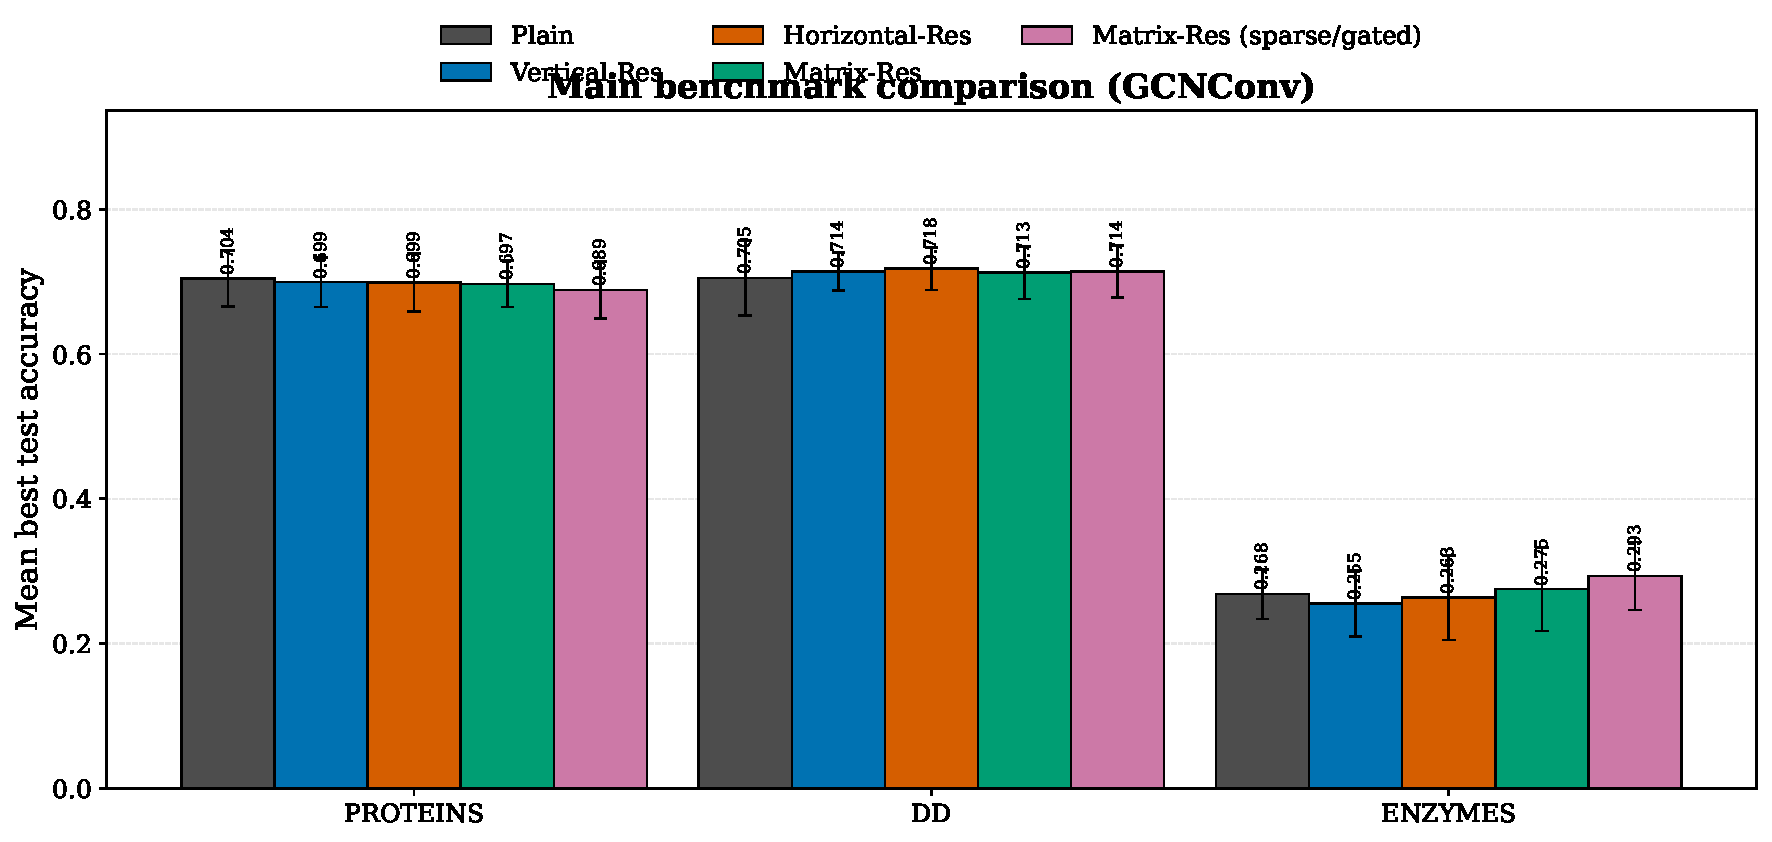
\includegraphics[width=0.92\linewidth]{figures/exp/fig_main_benchmark_gcnconv.pdf}
\caption{Main GCNConv benchmark at \(B=3\). Bars show five-fold mean best test accuracy with fold-level standard-deviation error bars.}
\label{fig:main_benchmark}
\end{figure}

Figure~\ref{fig:main_benchmark} makes the split regime visually explicit. The default GCNConv setting does not support a universal residual winner; instead, each dataset favors a different residual neighborhood.

\subsection{Operator robustness}

The full four-operator benchmark tests whether the GCNConv pattern is operator-specific. Table~\ref{tab:operator_wins} counts the winning topology across the 24 dataset--operator combinations. MatrixRes is the most frequent winner overall and wins under every operator family, but the remaining wins are distributed across all other models. This confirms that the residual-topology question is not reducible to one backbone choice.

\begin{table}[h]
\centering
\small
\caption{Winner counts across 24 dataset--operator combinations.}
\label{tab:operator_wins}
\begin{tabular}{l c c}
\toprule
Model & Wins & Mean rank \\
\midrule
Plain & 5 & 3.04 \\
VerticalRes & 2 & 3.38 \\
HorizontalRes & 3 & 3.54 \\
MatrixRes & \(\mathbf{9}\) & \(\mathbf{2.13}\) \\
MatrixResGated & 5 & 2.92 \\
\bottomrule
\end{tabular}
\end{table}

\begin{figure}[H]
\centering
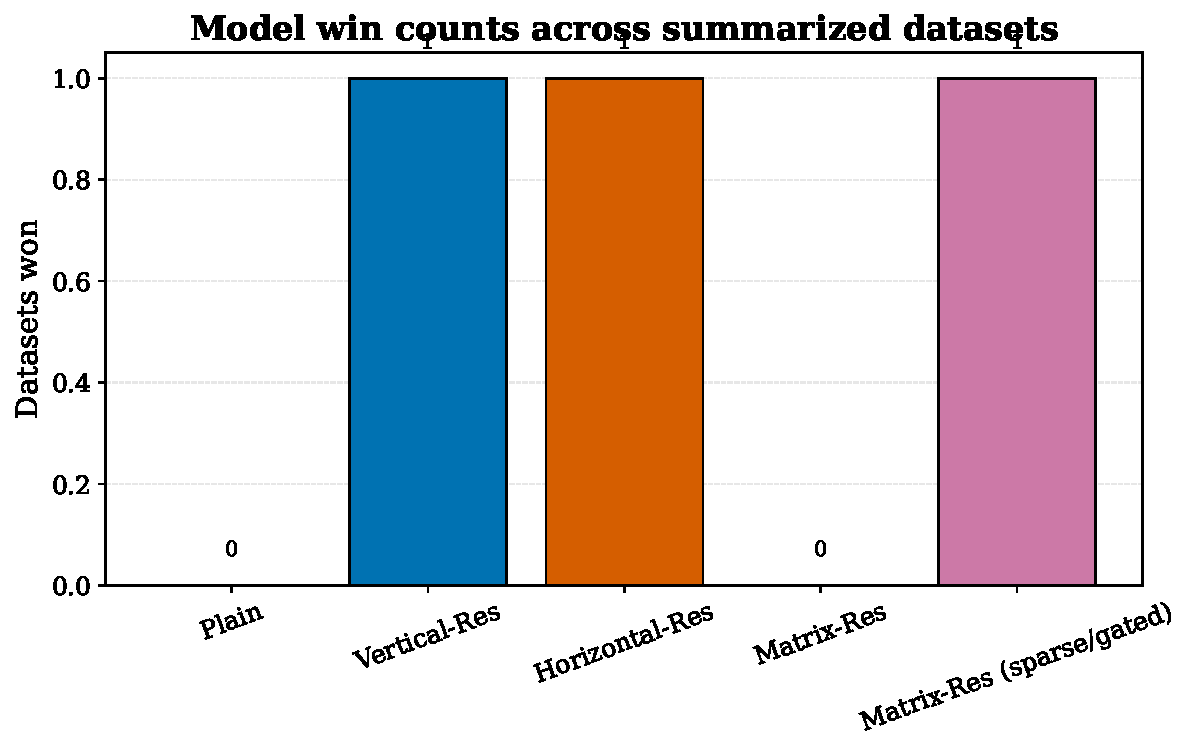
\includegraphics[width=0.82\linewidth]{figures/exp/fig_model_win_counts.pdf}
\caption{Model-level winner counts across the six datasets and four message-passing operators.}
\label{fig:model_win_counts}
\end{figure}

\subsection{Branch-count ablation}

Branch count has a non-monotonic effect. Table~\ref{tab:branch_best} reports the best branch count for each topology in the ablation. On PROTEINS, HorizontalRes peaks at \(B=4\), MatrixRes peaks at \(B=6\), and MatrixResGated peaks at \(B=3\). On DD, the preferred branch budget is smaller: HorizontalRes and MatrixRes peak at \(B=2\), while MatrixResGated is strongest at \(B=1\).

\begin{table}[h]
\centering
\small
\caption{Best branch-count setting for each topology in the ablation.}
\label{tab:branch_best}
\begin{tabular}{l l c c}
\toprule
Dataset & Model & Best \(B\) & Accuracy \\
\midrule
PROTEINS & HorizontalRes & 4 & \(0.7125\pm0.0286\) \\
PROTEINS & MatrixRes & 6 & \(0.7062\pm0.0210\) \\
PROTEINS & MatrixResGated & 3 & \(0.7098\pm0.0219\) \\
DD & HorizontalRes & 2 & \(0.7275\pm0.0304\) \\
DD & MatrixRes & 2 & \(0.7206\pm0.0411\) \\
DD & MatrixResGated & 1 & \(0.7283\pm0.0244\) \\
\bottomrule
\end{tabular}
\end{table}

\begin{figure}[H]
\centering
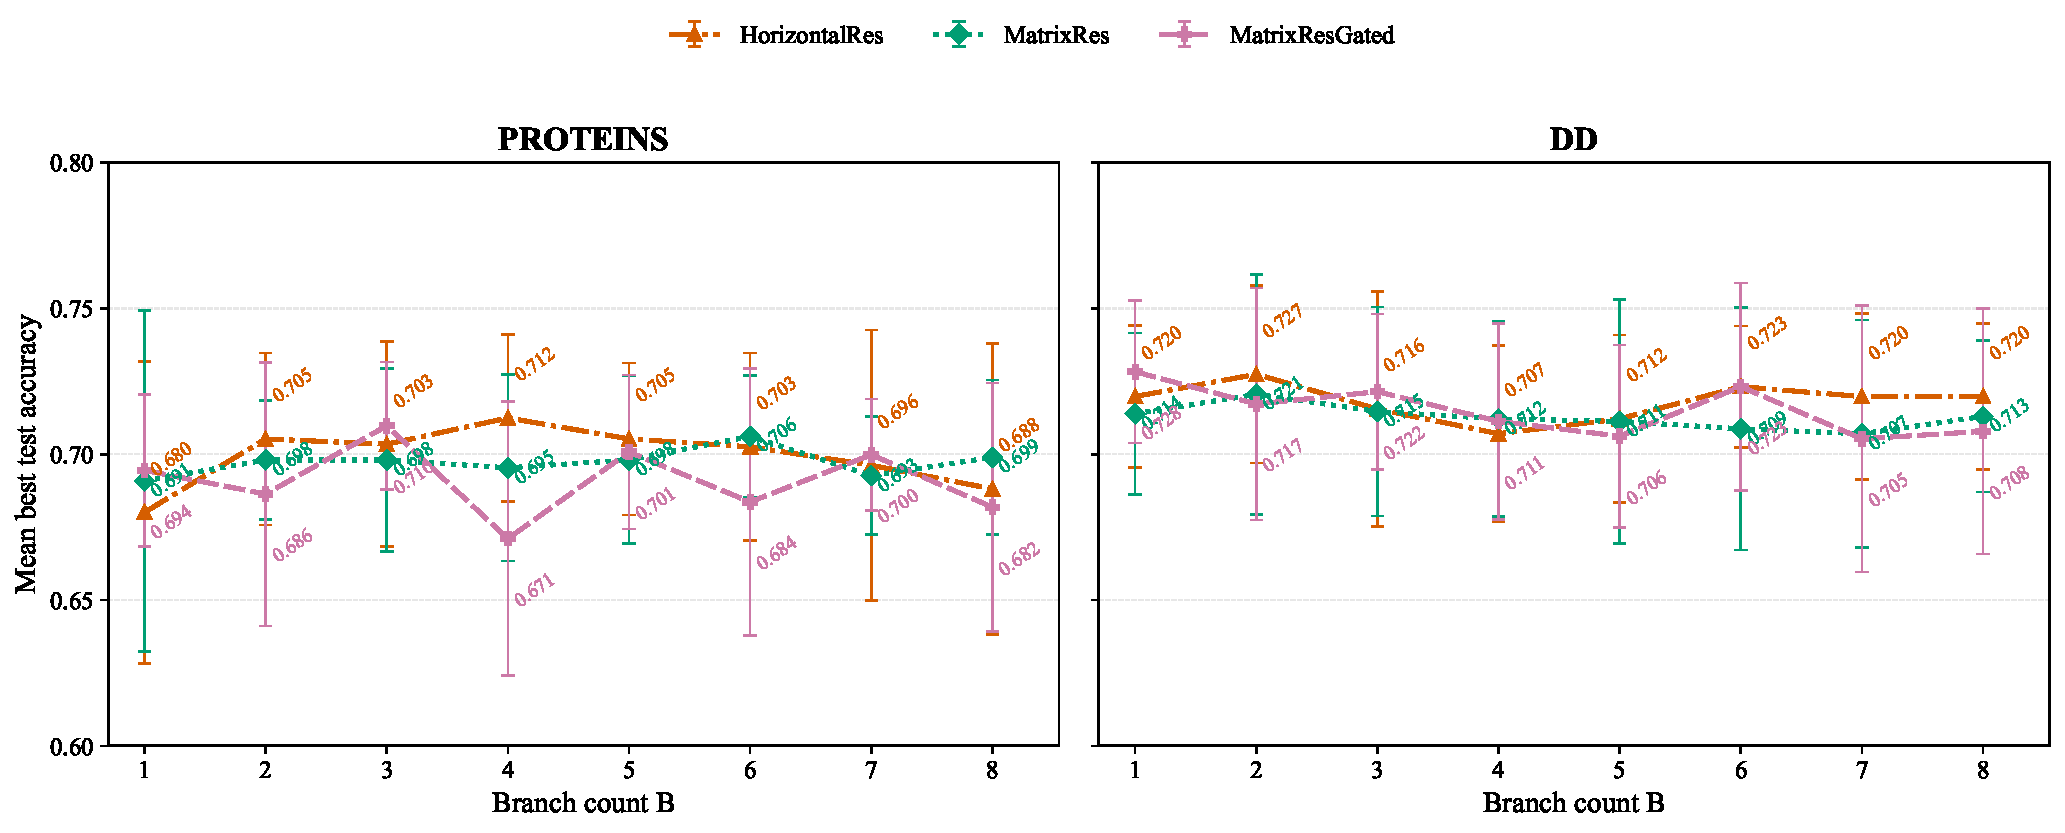
\includegraphics[width=0.92\linewidth]{figures/exp/fig_branch_count_ablation.pdf}
\caption{Branch-count ablation for HorizontalRes, MatrixRes, and MatrixResGated on PROTEINS and DD. Accuracy improves only within a useful operating region and then saturates or declines.}
\label{fig:branch_ablation}
\end{figure}

The ablation shows that branch count should not be read as a simple capacity knob. Increasing \(B\) changes the residual graph itself: it adds branches, residual paths, residual traffic, and optimization interactions. PROTEINS tolerates a moderate branch budget, while DD is more sensitive to redundant branch expansion.

\subsection{MatrixResGated sensitivity}

The fold-0 sensitivity scan shows that MatrixResGated is tunable, but its preferred region differs between datasets. On PROTEINS, the baseline MatrixResGated configuration reaches \(0.6726\), and mild sparsification with \(\lambda=0.02\) improves fold-0 accuracy to \(0.6951\). Stronger sparsification with \(\lambda=0.1\) reduces accuracy to \(0.6278\). On DD, the baseline fold-0 score is \(0.7300\), while \(lr=0.001\), \(dim=32\), and \(gate\_init=0.2\) each reach \(0.7511\).

\begin{table}[h]
\centering
\small
\caption{Strongest MatrixResGated fold-0 sensitivity settings.}
\label{tab:sensitivity}
\begin{tabular}{l l c l}
\toprule
Dataset & Setting & Accuracy & Interpretation \\
\midrule
PROTEINS & baseline & 0.6726 & default controlled matrix reuse \\
PROTEINS & \(\lambda=0.02\) & 0.6951 & mild sparsification improves fold 0 \\
PROTEINS & \(\lambda=0.1\) & 0.6278 & strong sparsification is harmful \\
DD & baseline & 0.7300 & default controlled matrix reuse \\
DD & \(lr=0.001\) & 0.7511 & conservative optimization helps \\
DD & \(dim=32\) & 0.7511 & smaller hidden dimension helps \\
DD & \(gate\_init=0.2\) & 0.7511 & lower initial gate helps \\
\bottomrule
\end{tabular}
\end{table}

\begin{figure}[H]
\centering
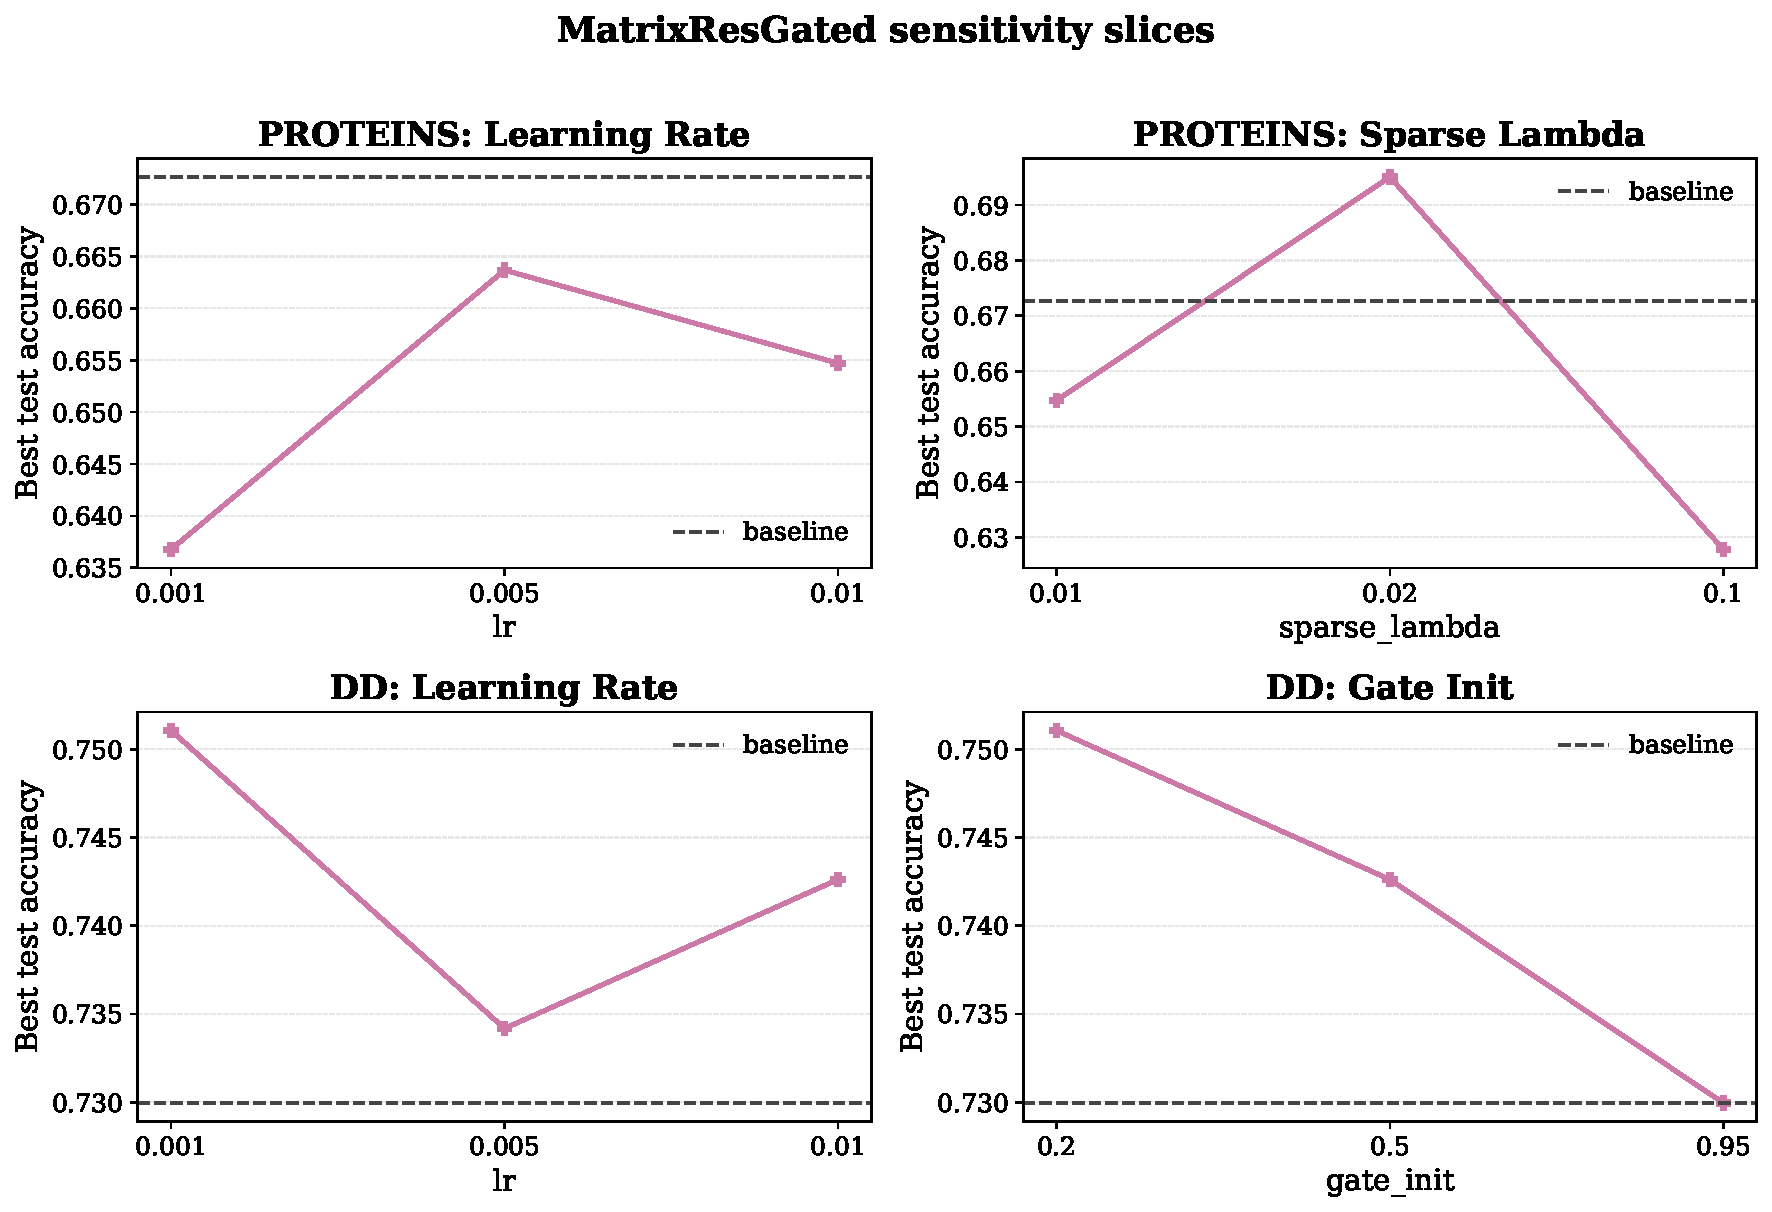
\includegraphics[width=0.92\linewidth]{figures/exp/fig_matrixresgated_sensitivity.pdf}
\caption{Fold-0 MatrixResGated sensitivity scan at \(B=3\). The scan identifies candidate operating regions but is not treated as final hyperparameter evidence.}
\label{fig:sensitivity}
\end{figure}

\subsection{Five-fold check of tuned MatrixResGated candidates}

To distinguish candidate discovery from evaluation, selected MatrixResGated settings were rerun across all five folds. Table~\ref{tab:tuned_candidates} reports these follow-up checks. On DD, the smaller hidden dimension is the strongest tuned candidate, reaching \(0.7215\pm0.0330\) while reducing parameters from 42,371 to 15,043. The lower learning rate is essentially tied with the default MatrixResGated benchmark, and the lower gate initialization is weaker. On PROTEINS, \(\lambda=0.02\) reaches \(0.6909\pm0.0447\), below the default MatrixResGated result, showing that the fold-0 sparsity gain is not stable across all folds in the current run.

\begin{table}[h]
\centering
\small
\caption{Five-fold checks of selected MatrixResGated candidates.}
\label{tab:tuned_candidates}
\begin{tabular}{l l c c c}
\toprule
Candidate & Dataset & Accuracy & Mean loss & Parameters \\
\midrule
\texttt{PROTEINS\_sparse\_lambda\_0.02} & PROTEINS & \(0.6909\pm0.0447\) & 0.6104 & 38,339 \\
\texttt{DD\_lr\_0.001} & DD & \(0.7181\pm0.0336\) & 0.5737 & 42,371 \\
\texttt{DD\_dim\_32} & DD & \(\mathbf{0.7215\pm0.0330}\) & 0.5717 & 15,043 \\
\texttt{DD\_gate\_init\_0.2} & DD & \(0.7131\pm0.0213\) & 0.5820 & 42,371 \\
\bottomrule
\end{tabular}
\end{table}

\subsection{Mechanism analysis}

The mechanism summaries support a common explanation for the rise-then-fall trend. Increasing branch count initially creates useful diversity: branches become less identical and can cover complementary feature subspaces. Past the useful regime, diversity alone is not sufficient. Residual traffic grows quickly, branch similarity may remain high, and gradient norms can weaken.

For HorizontalRes on PROTEINS, moving from \(B=1\) to \(B=4\) increases branch diversity from 0.0000 to 1.1450, while branch cosine decreases from 1.0000 to 0.8417. This corresponds to the accuracy improvement. Beyond \(B=4\), diversity continues increasing, reaching 1.5441 at \(B=8\), but accuracy declines to 0.6881. MatrixRes shows a similar trend at a larger branch budget, peaking at \(B=6\). DD is more conservative: branch expansion beyond \(B=2\) often adds residual complexity without enough functional separation.

\begin{figure}[H]
\centering
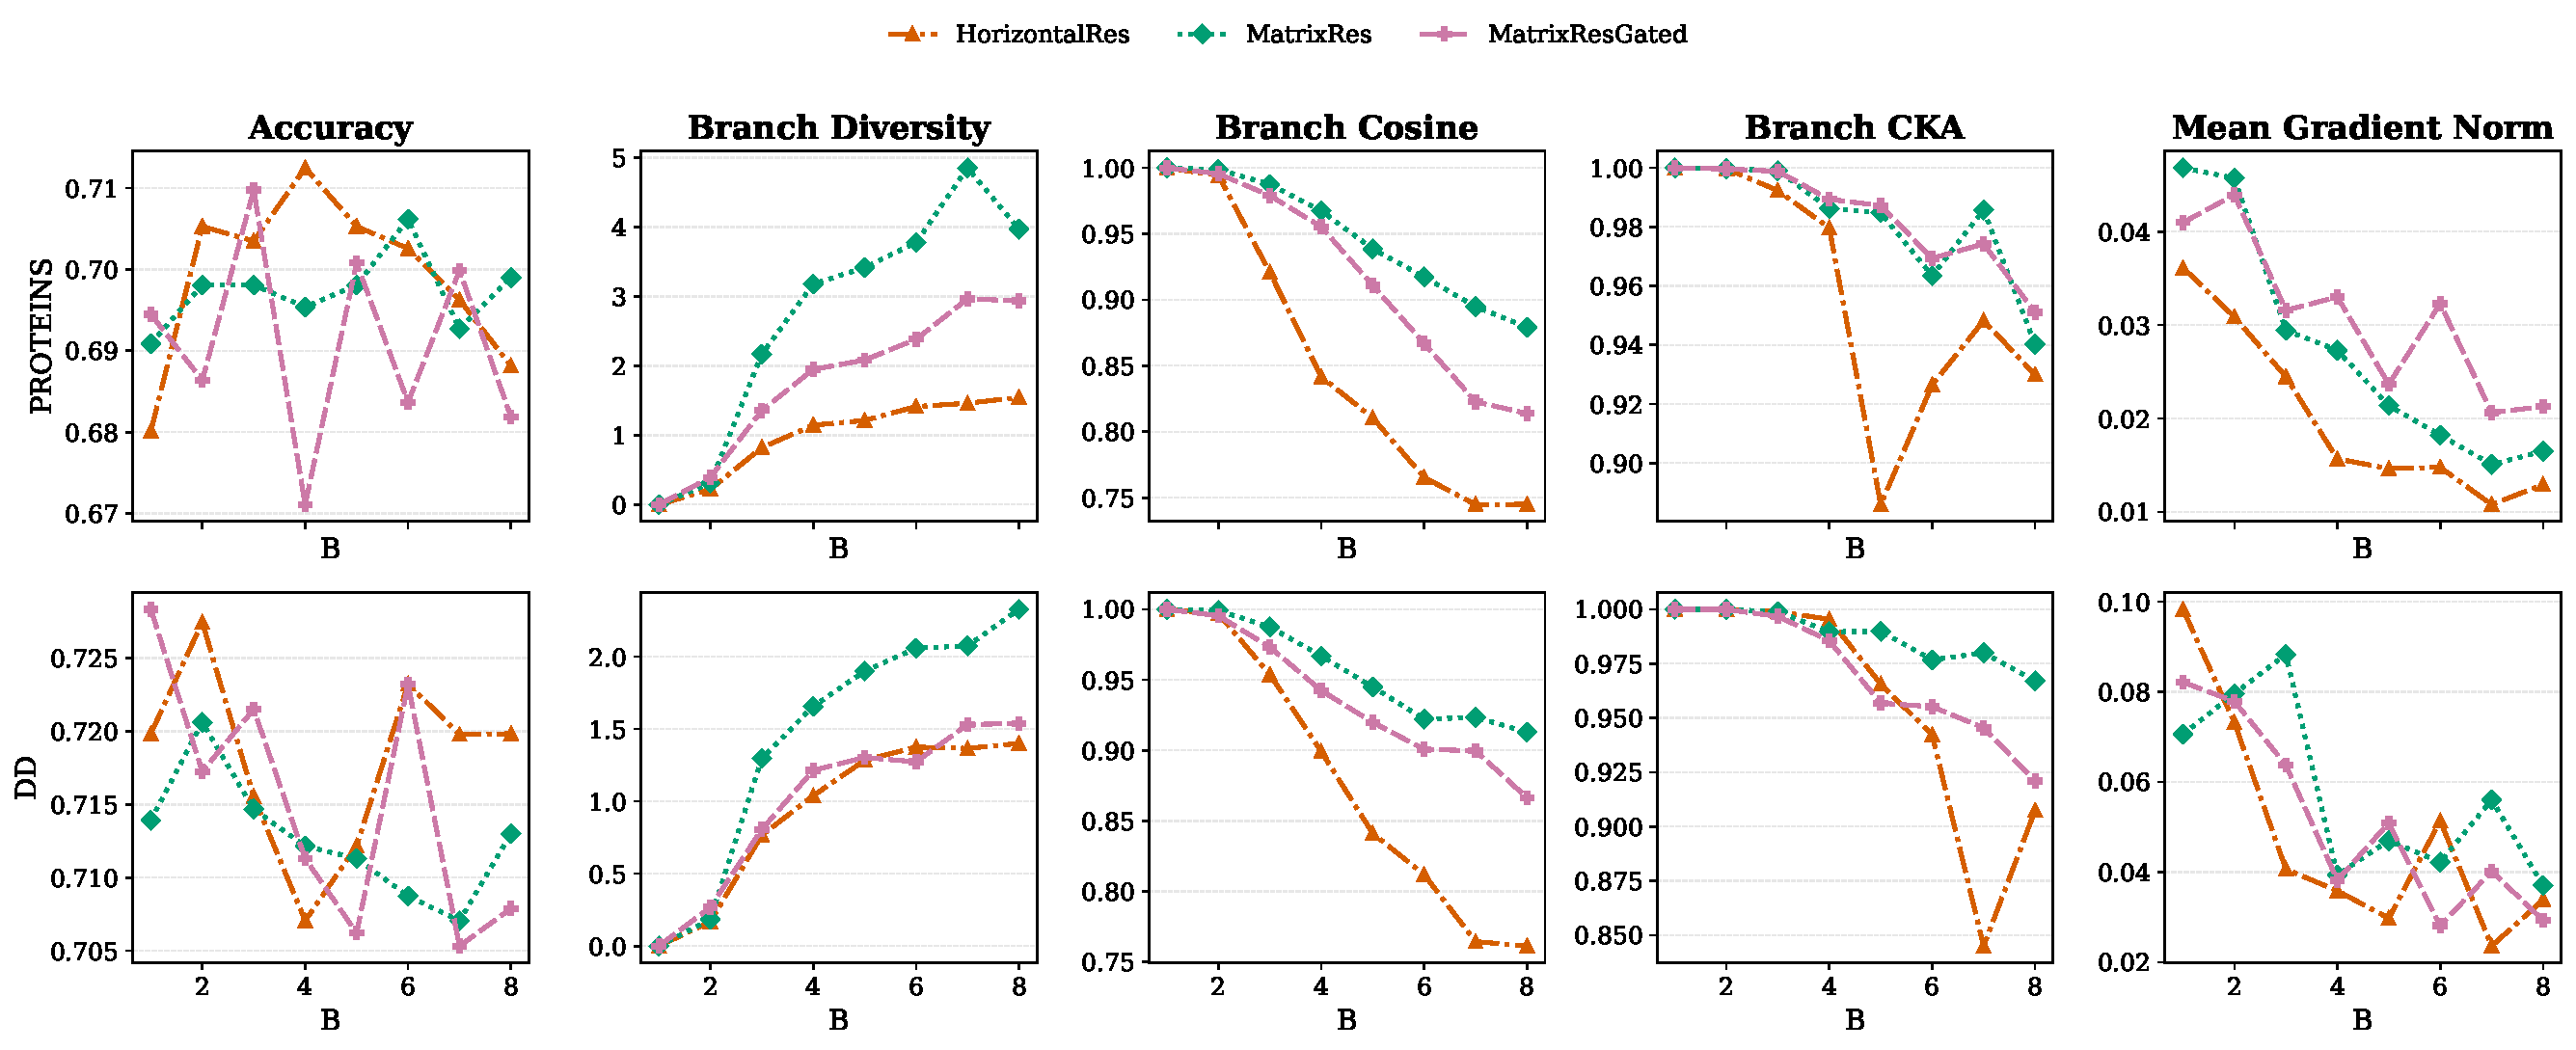
\includegraphics[width=0.92\linewidth]{figures/exp/fig_mechanism_branch_dynamics.pdf}
\caption{Mechanism summary linking branch-count accuracy to branch diversity, branch cosine similarity, and mean gradient norm.}
\label{fig:mechanism}
\end{figure}
